\documentclass{article}

\usepackage{amsmath, amsfonts, amssymb, amsthm}
\usepackage{hyperref}
\usepackage{float, tikz, caption}

\setlength{\parindent}{0pt}
\setlength{\parskip}{5pt}

\newcommand{\N}{\mathbb{N}}
\newcommand{\Z}{\mathbb{Z}}
\newcommand{\cP}{\mathcal{P}}

\title{IMO 2014 C4}
\author{}
\date{}

\begin{document}

\maketitle



\subsection*{Problem}

Let $\N^2$ be the set of non-negative lattice points, a.k.a. pairs of non-negative integers.
A \emph{skew-tetromino} in $\N^2$ is a subset of size $4$ that falls into one of the following type:
\begin{itemize}
    \item   Type 1: $\{(a, b), (a + 1, b), (a + 1, b + 1), (a + 2, b + 1)\}$ for some $a, b \in \N$,
    \item   Type 2: $\{(a + 1, b), (a + 1, b + 1), (a, b + 1), (a, b + 2)\}$ for some $a, b \in \N$,
    \item   Type 3: $\{(a, b + 1), (a + 1, b + 1), (a + 1, b), (a + 2, b)\}$ for some $a, b \in \N$,
    \item   Type 4: $\{(a, b), (a, b + 1), (a + 1, b + 1), (a + 1, b + 2)\}$ for some $a, b \in \N$.
\end{itemize}

\begin{figure}[H]
\centering
\begin{minipage}{.25\linewidth}
    \centering
    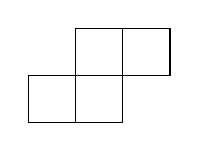
\begin{tikzpicture}
        \draw (0, 0) rectangle ++(0.6, 0.6);
        \draw (0.6, 0) rectangle ++(0.6, 0.6);
        \draw (0.6, 0.6) rectangle ++(0.6, 0.6);
        \draw (1.2, 0.6) rectangle ++(0.6, 0.6);
    \end{tikzpicture}
    \caption*{Type 1}
\end{minipage}
\begin{minipage}{.2\linewidth}
    \centering
    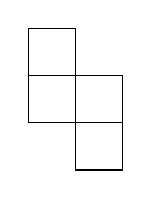
\begin{tikzpicture}
        \draw (0.6, 0) rectangle ++(0.6, 0.6);
        \draw (0.6, 0.6) rectangle ++(0.6, 0.6);
        \draw (0, 0.6) rectangle ++(0.6, 0.6);
        \draw (0, 1.2) rectangle ++(0.6, 0.6);
    \end{tikzpicture}
    \caption*{Type 2}
\end{minipage}
\begin{minipage}{.2\linewidth}
    \centering
    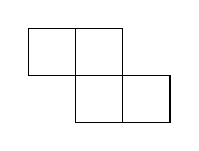
\begin{tikzpicture}
        \draw (0, 0.6) rectangle ++(0.6, 0.6);
        \draw (0.6, 0.6) rectangle ++(0.6, 0.6);
        \draw (0.6, 0) rectangle ++(0.6, 0.6);
        \draw (1.2, 0) rectangle ++(0.6, 0.6);
    \end{tikzpicture}
    \caption*{Type 3}
\end{minipage}
\begin{minipage}{.25\linewidth}
    \centering
    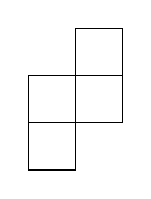
\begin{tikzpicture}
        \draw (0, 0) rectangle ++(0.6, 0.6);
        \draw (0, 0.6) rectangle ++(0.6, 0.6);
        \draw (0.6, 0.6) rectangle ++(0.6, 0.6);
        \draw (0.6, 1.2) rectangle ++(0.6, 0.6);
    \end{tikzpicture}
    \caption*{Type 4}
\end{minipage}
\end{figure}

Consider a multiset $S$ of lattice points in $\N^2$.
A \emph{skew-tetromino tiling} of $S$ is a partition of $S$ into skew-tetrominoes as a multiset.
In particular, for each $(a, b) \in \N^2$, the number of skew-tetrominoes in the partition is exactly equal to the number of occurrences of $(a, b)$ in $S$.

Given a tiling $\cP$ of $S$ and $i \in \{1, 2, 3, 4\}$, let $\pi_{\cP, i}$ denote the number of skew-tetrominoes of type $i$ used in $\cP$.
Prove that given any two tilings $\cP_1$ and $\cP_2$ of $S$ and an index $i \in \{1, 2, 3, 4\}$, $\pi_{\cP_1, i}$ and $\pi_{\cP_2, i}$ have the same parity.
That is, the parity of the number of skew-tetrominoes used in the tiling of $S$ of each type is an invariant of $S$.



\subsection*{Solution}

Official solution: \url{https://www.imo-official.org/problems/IMO2014SL.pdf}

We follow Solution 2, but we will repeatedly use the same idea for each skew-tetromino types.

Given $(x, y) \in \Z^2$, define the weight function $f_{x, y} : \N^2 \to \Z$ by $w_{x, y}(a, b) = x^a y^b$ for all $a, b \in \N$.
The total $(x, y)$-weight $w_{x, y}(S)$ of a multiset $S$ of $\N^2$ is defined by
\[ w_{x, y}(S) := \sum_{(a, b) \in S} f_{x, y}(a, b) = \sum_{(a, b) \in S} x^a y^b, \]
    where the sums are counted with multiplicity.
In our solution, $x$ and $y$ will be non-negative.

Next, we denote the skew-tetrominoes as follows:
\begin{itemize}
    \item   $T_{1, (a, b)} = \{(a, b), (a + 1, b), (a + 1, b + 1), (a + 2, b + 1)\}$,
    \item   $T_{2, (a, b)} = \{(a + 1, b), (a + 1, b + 1), (a, b + 1), (a, b + 2)\}$,
    \item   $T_{3, (a, b)} = \{(a, b + 1), (a + 1, b + 1), (a + 1, b), (a + 2, b)\}$,
    \item   $T_{4, (a, b)} = \{(a, b), (a, b + 1), (a + 1, b + 1), (a + 1, b + 2)\}$.
\end{itemize}

By direct computation, one obtains
\begin{align*}
    w_{x, y}(T_{1, (a, b)}) &= (x + 1)(xy + 1) x^a y^b, \\
    w_{x, y}(T_{2, (a, b)}) &= (y + 1)(x + y) x^a y^b, \\
    w_{x, y}(T_{3, (a, b)}) &= (x + 1)(x + y) x^a y^b, \\
    w_{x, y}(T_{4, (a, b)}) &= (y + 1)(xy + 1) x^a y^b.
\end{align*}
As in the official solution, the main idea is as follows.
Fix one index $i \in \{1, 2, 3, 4\}$ for a skew-tetromino type.
If we choose a suitable $x$ and $y$, then the weight of any skew-tetromino of type other than $i$ is divisible by some positive integer $n$.
But $n$ never divides the weight of skew-tetrominoes of type $i$.
In fact, the weight modulo $n$ will also be invariant that does not depend on the exact position of the skew-tetromino.

We pick $n = 2 \cdot 16 = 32$.
For each $i \in \{1, 2, 3, 4\}$, we choose $x_i, y_i \in \N$ such that the weight $w_{x_i, y_i}$ of type $i$ skew-tetrominoes are always $16 \pmod{32}$.
Also, the corresponding weight of any other type of skew-tetrominoes are divisible by $32$.
Then $16 \pi_{\cP, i} \equiv w_{x_i, y_i}(S) \pmod{32}$ always holds for any partition $\cP$ of $S$.
In particular, the parity of $\pi_{\cP, i}$ will be an invariant of $S$.
The choice of $x_i$ and $y_i$ are done case-by-case:
\begin{itemize}
    \item   $x_1 = 13$, $y_1 = 3$,
    \item   $x_2 = 3$, $y_2 = 5$,
    \item   $x_3 = 5$, $y_3 = 3$,
    \item   $x_4 = 3$, $y_4 = 13$.
\end{itemize}



\subsection*{Extra notes}

The above version is a very generalized version of the original problem.
In the original problem, $S$ is a proper set; every lattice points in $S$ has multiplicity $1$.
Furthermore, the question assumes that there is a tiling $\cP$ with $\pi_{\cP, 3} = \pi_{\cP, 4} = 0$.
Then it asks to prove that given any tiling $\cP$ of $S$, $\pi_{\cP, 3} + \pi_{\cP, 4}$ is always even.

In the implementation, we simply further.
We remove the occurrence of $S$; we just assume that the sum of the multisets in $\cP_1$ and $\cP_2$ are equal.
By sum over multisets, we mean the union, counting multiplicities.



\end{document}
